
%(BEGIN_QUESTION)
% Copyright 2010, Tony R. Kuphaldt, released under the Creative Commons Attribution License (v 1.0)
% This means you may do almost anything with this work of mine, so long as you give me proper credit

Analyze this Siemens S7-200 PLC program (for controlling a motor) and explain what it is supposed to do:

$$\includegraphics[width=15.5cm]{i02255x01.eps}$$

Include an explanation of the motor contactor wiring, based on an analysis of the PLC program.

\vfil

\underbar{file i02255}
\eject
%(END_QUESTION)





%(BEGIN_ANSWER)

This is a graded question -- no answers or hints given!

%(END_ANSWER)





%(BEGIN_NOTES)

The standard Start, Stop, and Seal-in contact structure in this program should remind you of every PLC-controlled motor system program you've ever seen.  The ``twist'' here is that the {\tt M0.2} bit does not directly control the motor, but rather must be enabled by another bit ({\tt T6}) to energize any real-world output channels.  Depending on the state of this {\tt T6} bit, either the Low-speed ({\tt Q0.0}) or the High-speed ({\tt Q0.1}) outputs will be energized, but never both simultaneously.

\vskip 10pt

Thus, this is a two-speed motor start-stop control system, which starts the motor at low speed for 5 seconds then shifts to high speed.  The motor continues to run in High-speed mode until it is stopped by de-energizing the {\tt I0.5} ``Stop'' input (which tells us the Stop pushbutton must be wired normally-closed).  

The motor control circuit -- although not shown to you here -- uses two contactors: one for low speed and another for high speed.  We cannot tell exactly how they are wired, perhaps using a star-delta strategy for two-speed operation or perhaps using resistors in the low-speed mode.

%INDEX% PLC, ladder logic program analysis and explanation

%(END_NOTES)



